
\renewcommand{\footerfilename}{Install.tex}

\section{Critical First Steps}

Currently there are too many ways to install IRAF/Pyraf.

One package demands an \dhl{/etc/iraf} directory that has a file called \dhl{irafroot}
with the contents:
\begingroup \fontsize{10pt}{10pt}
\selectfont
\begin{verbatim} 
/opt/iraf/lib/iraf/
\end{verbatim}
\endgroup
It may way want a copy of \dhl{login.cl} at that location.

Some packages expect:

\dhl{\$HOME/iraf}

\dhl{\$HOME/.iraf   \# hidden}

in order to find the loginuser.cl directory.

The real answer is to put everything iraf/pyraf related into

\dhl{/opt/iraf} under appropriate subdirectories.

This is spelled out in the \dhl{Filesystem Hierarchy Standard} \index{Unix!file hierarchy}.

\url{https://wiki.linuxfoundation.org/lsb/fhs}.


It is critical you properly install the IRAF/PyRAF3 packages. This
release looks for a {\textasciitilde}/.iraf directory that may not be fully integrated
into the rest of IRAF.

You may make a soft link of \dhl{\home/iraf} to \dhl{\home/.iraf}:

\dhl{ln -s \home/iraf \home/.iraf}

The document will continue to refer to \dhl{\home/iraf} as the base
of the IRAF package. 

It is important to use a \dhl{~/iraf/loginuser.cl} file with task
aliases foreign and tasks.\index{tasks!aliases} \index{tasks!foreign
  tasks}

One way to make things simple is to create a bash alias for PyRAF that:
\vspace{-.15cm}
\begin{enumerate}\addtolength{\itemsep}{-0.5\baselineskip}
%\setcounter{enumi}{N}
   \item   uses xdotool to change the color of the window's background
   \item   update the PATH and PYTHONPATH to access all the special files you use
   \item   run the system pyraf (note the /usr/bin path is prefix is necessary) 
 with the ``-s'' switch for ``silent'' start.
\end{enumerate}


\begingroup \fontsize{10pt}{10pt}
\selectfont
%%\begin{Verbatim} [commandchars=\\\{\}]
\begin{verbatim} 
alias pyraf="xdotool key shift+F10 r 1;\\
  export PATH="/usr/local/bin:$PATH"; export PATH="/usr/local/astrometry/bin:$PATH";\\
  export PYTHONPATH=$HOME/.iraf; export PATH="$HOME/.iraf/smtsci/bin:$PATH";\\
  /usr/bin/pyraf -s;"
\end{verbatim}
\endgroup
%% \end{Verbatim}

\subsection{IRAF/PyRAF Tasks and Packages}

IRAF, from ye-olden times, uses \dhl{packages} containing help text
and parameter files to hold values from run-to-run together with the tasks'
executable code.
\index{IRAF!tasks} Tasks are ``programs'', usually written in FORTRAN
or in cl proceedural code. Some are written in C/C++.

\dhl{BEWARE}: IRAF is \dhl{sticky}! It retains parameter values from
run-to-run that can perpetuate errors. Review all the parameters to be
sure your reductions are proper. These values are stored in the
\dhl{~/iraf/uparm} directory.

Tasks are built into IRAF/PyRAF but are only loaded once. Each time
they are used -- they are in memory and already part of the CPU thread
you are using. Thus they very fast. Using \llbox{!} shell-escape or a
\dhl{\$foreign} task causes Unix to create a new heavy-thread with
significant overhead (especially in a loop).

IRAF has a habit of loading images into memory and keeping them there.
Some tasks will modify the in-memory image but not write it back to
the disk. Work may be lost. See Section \ref{sec:FITSFiles} for quick
details.

IRAF has a neurotic habit of \dhl{sometimes} adding an extent to
certain FITS files! This is the case with master darks and flats
and a handful of other operations.

It is best to develop your \dhl{reduce.pyraf} script in an editor, one line
and step at a time, then cut/paste edited lines at the interactive
prompt. When you make a mistake -- and you will -- you can start over
with a fresh copy of data and stop short of the mistake. Pick up and
go again.

\subsection{Full On Python Hacks}

\example Python's \dhl{import iraf} statement allows for operations like: \\
\prose I want to use IRAF's imstat command to get a binary value, assign
the value to my python variable. \\
\exercise Enter: \\
{\color{verbcolor}{
\begingroup \fontsize{10pt}{10pt}
\selectfont
%%\begin{Verbatim} [commandchars=\\\{\}]
\begin{verbatim} 
mymean = float( iraf.imstat(images='*fits',fields='mean',format=iraf.no,Stdout=1)[0])
\end{verbatim}
\endgroup
%% \end{Verbatim}
}}

\takeaway The task has a pythonic wrapper, contained in the iraf.py
module's namespace.  It needs a list of files, we only want the one
field \dhl{mean}, we do not want the headers (format=iraf.no). The
phrase Stdout=1 (note capitalization) returns the text as a string
rather than printing on the terminal. But! The string is actually an
array, so we want the first bit. But! that bit is a string, and we
need to convert to binary with the \dhl{float} python function.

where \dhl{mymean} is now a proper python float. Yes, convoluted, but
its buried in a scrip and available for your use. \index{Stdout}

\subsection{Task Parameters}

Always be aware of the:
\vspace{-.15cm}
\begin{enumerate}\addtolength{\itemsep}{-0.5\baselineskip}
%\setcounter{enumi}{N}
   \item    ~/iraf/uparm directory
   \item    lparm <taskname> command to list parameters.
   \item    \dhl{unlearn <task>} command.
   \item   help <task> and look at the see also part at the bottom.
\end{enumerate}

\section{Goals}

The main goal of scripting is not the script, it is the result. Good
data results do not come from good scripting -- but come from good
planning, good execution of the plan and attention to configuring
your tools.


\subsection{Things to remember}

IRAF \dhl{cl} morphed into PyRAF \cite{2006hstc.conf..437G} to allow a more
powerful \dhl{cl} by hacking the Python \dhl{readline} subsystem. The
grammar of python was altered to allow for a ``direct entry'' of most older
\dhl{cl} commands. Direct access to the underlying tasks was
accomplished with a ``cythonic'' interface into underlying code. An ``iraf''
module was added to support programming calls to IRAF tasks and using 
a special Python \dhl{keyword} argument Stdout to return output as a string.
Parsing this string with python allows chaining \dhl{cl} commands together
for a goal.

A tremendous amount of power is available for you to mix and match to meet
your specific needs. 

\subsection{Observation Directory}

One can not expect proper structure by simply importing a night's
observations, warts blisters and all. Files will be scattered all
over, mis-named, bad headers, useless(!), and other oddities. But copy
the data into date/RawData. See directory layout table \ref{figure:dirlayout}

Open date/usw/reduce.cl in your favorite editor. Anything you want
to type into PyRAF -- type it into the reduce.cl file. Then cut/paste
the command to PyRAF. This means when you make the mistake -- you
can remove the last line, save the reduce.cl file, and rebuild
to that point. Yes, some interactive things will or may happen.
Try not to make too many mistakes.

\vspace{-.15cm}
\begin{enumerate}\addtolength{\itemsep}{-0.5\baselineskip}
   \item   cd ~/Observations
   \item   mkdir 22Feb2022 \# date of sunset at the observatory
   \item   cd 22Feb2022
   \item   mkdir -p Plan RawData PreAnalysis Analysis Publish usw
   \item   mkdir -p PreAnalysis/{Bias,Darks/{s300,s3},Flats,Comps} \# prior knowledge
   \item   cd RawData
   \item   cp -pr /mnt/NAS/22Feb2022/* .  \# copy the raw data
\end{enumerate}

Now the plan for observations and initial PreAnalysis results is in 
place. The \dhl{usw/reduce.cl} script is the key. 

Good observations are the result of good planning. Make the list of targets,
determine offsets and guide stars, create a ds9 region file in ICRF WCS
coordinates for the field of view and possible orientations of the instrument.
If possible download the preparation package from the observatory and take
time to prepare. \index{planning}

\begin{figure}[h!]
\centering
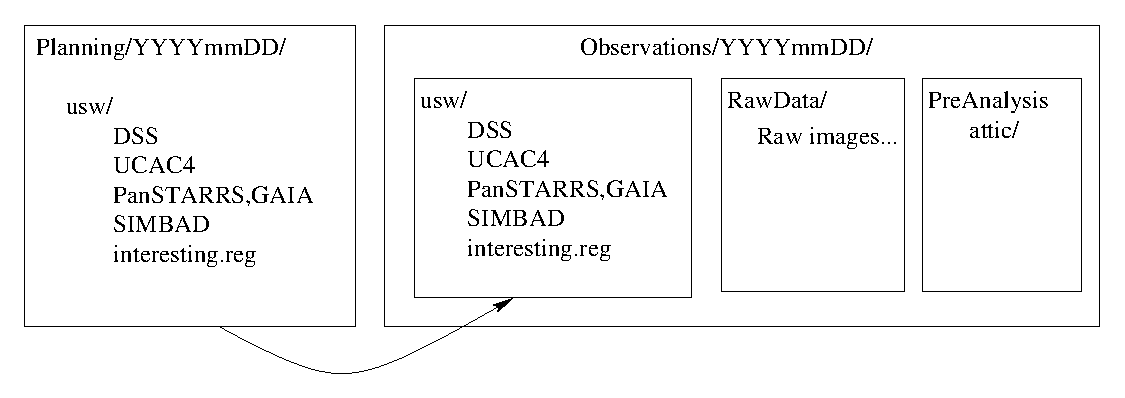
\includegraphics[width=.4\textwidth]{images/Overview.eps}
\caption{The observations directory was in place with the plan.
Load up the raw images. Then copy raw data to pre-analysis.} %% \caption{{\tiny{citation}}}
\label{figure:GoalsOverview}
\end{figure}

\clearpage
\subsection{The main tricks}

Note: Unix files do not rely on their extensions. A Unix extension is a social
convention. Many authors use two files, like \dhl{in.txt} and \dhl{out.txt}.
They will use an editor to change the bits of one to another. 

I recommend using goofy file names, like \dhl{xxx} and \dhl{l.l}, when seen
they may be removed. The filename \dhl{l.l} is real easy to type because
the \llbox{l} and \llbox{.} are right next to each other!

The \llbox{/}\llbox{/} sequence is the cl concatenation operator, used to
join two strings without intervening whitespace.

Instead of having the input files in in.txt, then editing to make unique
output names -- simply prepend a string, with some meaningful context
to the @file. 

The order of operations may be to
\vspace{-.15cm}
\begin{enumerate}\addtolength{\itemsep}{-0.5\baselineskip}
%\setcounter{enumi}{N}
   \item   t\_ trim a file.
   \item   c\_ cosmic ray removal
   \item   z\_ to zero correct
   \item   d\_ to dark correct
   \item   f\_ to flat a file
\end{enumerate}


etc. data.fits, after processing may be \dhl{f\_d\_z\_c\_t\_data.fits}.

So PyRAF has several tricks up its sleave:
\begin{itemize}
\addtolength{\itemsep}{-0.5\baselineskip}
   \item   It can act like a basic ``calculator'' just by typing standard python at the
PyRAF command prompt. Remember to ``import'' packages like math and numpy.
   \item It works with list of files. These are refered to as ``list''
     or ``at'' files. They are like {\color{verbcolor}{\verb#@l.l#}}
     where the file ``l.l'' has a list of filenames -- one per line.
   \item You can take the files in ``l.l'' and produce new files with
     the same name but prepend a clause to the
     filename!\\ \textbf{E.g.:}
     {\color{verbcolor}{\verb#imarith @l.l - zmaster.fits z_@l.l#}}\\ will
     subtract the zero master from each file in ``l.l'' and make a
     corresponding {\color{verbcolor}{\verb#z_filename.fits#}}.
\item PyRAF is a a replacement for {\color{verbcolor}{\verb#cl#}} (actually
ecl). You can loop {\color{verbcolor}{\verb#.cl#}} commands together
with bash commands into the mix to do work using:\\
{\color{verbcolor}{\verb#cl < ~/iraf/fit2fits.cl#}} to bring a Vendor's
fit format to the PyRAF standards.
\end{itemize}

It has a few oddities, inherited from the ecl lashup of the Pythonic 'readline' hack,
ripped from a \dhl{reduce.cl} script:

\vspace{-.15cm}
\begin{enumerate}\addtolength{\itemsep}{-0.5\baselineskip}
   \item Oops! Its Python 2.7 so write helpers like \dhl{trim} and
     \dhl{fitsls} accordingly.
   \item   Most of the IRAF \dhl{cl} commands work
   \item   \dhl{set OBSROOT=/home/me/Observations/23Feb2022}
   \item   \dhl{set OBS=OBSROOT\$/PreAnalysis}
\end{enumerate}

The IRAF command \dhl{chdir} \index{cl!chdir} changes directory while respecting
the IRAF use of iraf-environment variables.

You can escape to bash by starting the line with a bang (!). This
allows developing handy bash scripts to store in iraf/bin.

\clearpage

\subsection{System Setup}

I presume the use of the Ubuntu 22.04 Linux distribution from Canonical\texttrademark.

%% Under Microsoft Windows\texttrademark Pro, there is a system called \dhl{Hyper-V}.
%% It is very ``light-weight'' virtualization layer for Windows that permits
%% the seamless of an essentially containerized Ubuntu 22.04 + anaconda and other
%% Linux based tools while maintaining contact with the Windows file system,
%% the network etc. \index{Windows!Hyper-V}.

%%Under Linux you are running Linux anyway.
MacOS is very Linux like, even on their M1 processor series.

Install the Anaconda package without the Navigator. This brings in
a massive amount of power, including Astropy \cite{astropy:2013} \cite{astropy:2018}
\cite{astropy:2022}.
\vspace{-.15cm}
\begin{enumerate}\addtolength{\itemsep}{-0.5\baselineskip}
   \item    Necessary:
\vspace{-.15cm}
\begin{enumerate}\addtolength{\itemsep}{-0.5\baselineskip}
   \item    Ubuntu 22.04/Mac OS + many apt-get packages
   \item    Anaconda (Python 3+)
   \item    Astroconda PyRAF recipe (a python2.7 env)
   \item    Ubuntu aptitude iraf/pyraf packages
   \item    Sextractor
   \item    Current SAOImage/ds9
   \item    Current Astrometry.net + 4200 and GIAI data
   \item    Fitsverify \cite{fitsverify-1}
   \item    GitHUB sasiraf package (currently private contact author.)
\end{enumerate}
   \item    Optional
\end{enumerate}

\subsection{Unix\texttrademark Aliases}
A few aliases need to be setup.

\ltodo{Add Aliases}{Update/add aliases for bashrc file.}

\begin{figure}
{\color{darkred}
\begingroup \fontsize{10pt}{10pt}
\selectfont
%%\begin{Verbatim} [commandchars=\\\{\}]
\begin{verbatim} 
function pyraf  { #export PYTHONPATH=$HOME/iraf;
                  export PATH="/home/wayne/anaconda3.8/envs/geminiconda \\
                     /bin:$HOME/iraf/smtsci/bin:$PATH"; (folded line)
                  source activate geminiconda;
                  xdotool key shift+F10 r 6;     # change terminal color
                  $HOME/anaconda3/envs/geminiconda/bin/pyraf -s $*;
                }
\end{verbatim}
\endgroup
%% \end{Verbatim}
}
\caption{An entry into the aliases file, using the Gemini PyRAF installation.}
\label{fig:geminialias}
\end{figure}

This is a little-bit complicated:
\vspace{-.15cm}
\begin{enumerate}\addtolength{\itemsep}{-0.5\baselineskip}
   \item   The PYTHONPATH allows pyraflogin3 to be imported after start.
   \item   This assumes \dhl{~/iraf/pyraflogin.py} is present.
   \item   The function in figure \ref{fig:geminialias} tells Anaconda to activate
     the geminiconda environment
   \item   The xdotool allows the color of the terminal window to be changed.
   \item   PyRAF is then started, the \dhl{-s} switch is quiet about packages loaded.
   \item When PyRAF starts, it loads \dhl{login.cl} which in turn
     loads my \dhl{loginuser.cl} scripts.
\end{enumerate}

\subsection{Initialization files}

PyRAF uses \dhl{~/.iraf/login.cl} to manage system level commands and should
not be edited -- except to ensure that \dhl{cl < "home\$/iraf/loginuser.cl"} is
enabled. Edit the \dhl{loginuser.cl} file and pile changes.
 \index{Initialization!login.cl}
\index{Initialization!loginuser.cl}

A special \dhl{~/iraf/pyraflogin.py} file can 'extend' the Python
environment.  A sample file is available with this package. It
requires the special alias to start PyRAF. It adds simple
\dhl{matplotlib} plotting and some handy fixer-upper functions. See
that package for documentation. \index{Initialization!pyraflogin.py}

\subsection{Initial Steps}

This process uses a user-defined  directory structure as shown in
figure \ref{figure:basicpipeline}. 

The main steps are:
\vspace{-.15cm}
\begin{enumerate}\addtolength{\itemsep}{-0.5\baselineskip}
   \item   Layout basic directory structure:


   \item  Add a few toplevel soft-links for non-sentient file browsers.
\dirtree{%
.1 \$HOME/.aaatoday linked to \$HOME/Desktop/Today.
.1 \$HOME/.aaareduce linked to current working reduction.
}

   \item   Planning - load up the \dhl{\$HOME/Desktop/Today/usw} directory with
FOV files, and anything related to observatory etc.

   \item   Observe
   \item   Move dhl{\$HOME/Desktop/Today} to dhl{\$HOME/Desktop/Observations/mmDDDyyy}
date of sunset at the observatory of the instrument.
   \item   Make a safe backup.
   \item   Start the process of reducing the data.
\end{enumerate}

The script provides the audit trail you used. Modify this for each
instrument setup, and for each filter type etc.  Essentially the same
for spectroscopy -- just watch the statistics sections.

You may not need darks, and the flats will be different.

When, not if, you mess up you can delete the PreAnalysis directory, fix
the above script, and start over. As you move deeper into the file
processing, the script becomes more valuable.


\clearpage
\subsection{PyRAF Calculator Mode}

\goal Demonstrate borrow PyRAF as a calculator within PyRAF. Determine
the mean plus 3 times the standard deviation for a limit.

\example 
{\color{verbcolor}{\verb#imstat zmaster.fits fields=mean,stddev#}} \\
you find the mean is 346 and the stddev is 47.

\exercise How many pixels in the zero master are 3 or 5 $\sigma$ above
the mean?

{\color{verbcolor}
\begingroup \fontsize{10pt}{10pt}
\selectfont
%%\begin{Verbatim} [commandchars=\\\{\}]
\begin{verbatim}
from astropy import fits  # DO THE IMPORTS ONCE
import numpy

f = fits.open('zmaster.fits')    # open the fits file as a cfitsio like
d = f[0].data   # get the data   # structure and just grab the data.
# using some python magic!
(mean,stddev) = map(float,
                   iraf.imstatistics(Stdout=1,fields='mean,stddev',
                      images='zmaster.fits',format=iraf.no)[0].split())
len(d[d> mean + 3.0*(stddev)]) # 25729 pixels matched this example
len(d[d> mean + 5.0*(stddev)]) #  1220 pixels matched this example
f.close()
\end{verbatim}
\endgroup
%% \end{Verbatim}
}


\prose Hey, we're PyRAF, a pythonic interpreter -- so lets really use
Python.  The imports are used to get the modules/functions we
need. The fits.open gets the FITS file open for business; we grab just
the image data as a numpy array of shape
{\color{verbcolor}{\verb#NAXIS2,NAXIS1#}} (switched(!), numbered from
zero now and the data will have overscans if present!) using
{\color{verbcolor}{\verb#d = f[0].data#}}. The
{\color{verbcolor}{\verb#iraf#}} is imported by virtue of we're PyRAF;
the {\color{verbcolor}{\verb#imstat#}} is run as a python function
using {\color{verbcolor}{\verb#iraf.statistics()#}}.  The
{\color{verbcolor}{\verb#Stdout=1#}} tells the task to return the
output not send it to the terminal. The
{\color{verbcolor}{\verb#format=no#}} tells the function to omit the
usual header text etc, and just return the two values requested with
the {\color{verbcolor}{\verb#fields="mean,stddev"#}}.  The output is
one string with two ASCII numbers. These are split into an array, then
the {\color{verbcolor}{\verb#float#}} function converts the strings
into actual numbers -- returned as the tuple
{\color{verbcolor}{\verb#(mean,stddev)#}}.

\subsection{Using Numpy Arrays}
%HEREHEREHERE

Numpy arrays follow the ``C'' indexing scheme, which is ``ordinal'' in nature
(starting with zero). For an (X,Y,Z) index -- the array is referenced \dhl{backwards}:
myarray[Z][Y][X]. This differs from the FORTRAN convention for arrays, ``cardinal''
in nature (counting from 1).

FITS images are stored in FORTRAN order, and in Big Endian format. This makes
difficult for Intel architectures.

This is critical. Data are written into FITS images in so-called \dhl{Big-Endian}
fashion. In Jonathan's ``Gulliver's Travels'', a fictional character encounters
a culture in heated conflict over weather or not one should crack open an
egg on the little end or the big end. Computer aritectures are conflicted on
how to store a larger value, say an integer that spans more than one byte
into a linear address space. Decisions (bad perhaps) were made to store
a 16-bit integer with the byte containing least significant digit first.
The word oxBO is stored with the 0 first then the 0x0B. This was to make
a very early machine fast at ++value operations! We're stuck with that decision
since.

The real issue boils down to the Bad Thing\texttrademark practice of
``type punning'' whereby a block of data in ``Endianess Be Damed''
format is read into memory, then attempts to access it as though it
had the right byte order results in catastropy when data is exchanged
between the types of architectures.

Intel processors are ``Little Endian'' where processors like the Motorla
68000 were ``Big Endian''. 

Data are stored as arrays, with astropy.fits.io open command setting the
data[0] extent as a pythonic numpy array. So the indices are a bit backwards
The fits header would read something like:

\begingroup \fontsize{10pt}{10pt}
\selectfont
%%\begin{Verbatim} [commandchars=\\\{\}]
\begin{verbatim} 
NAXIS  = 2
NAXIS1 = 2048
NAXIS2 = 512
\end{verbatim}
\endgroup
%% \end{Verbatim}

To store a 2D image array. This is ment to denote an image that is 2048 wide and 512
tall. 

\ltodo{numpy vs FORTRAN}{Get into index details.}


The next bits use numpy arrays. Here we use the conditonal indexing
mode common to numpy arrays to get all the pixels that match
expression of the value > the
{\color{verbcolor}{\verb#mean + n times stddev#}}.

Need a ``Quick Calculation'' to find the center of an image to
use as a ``statistics section'' for normalizing?:

{\color{verbcolor}
\begingroup \fontsize{10pt}{10pt}
\selectfont
%%\begin{Verbatim} [commandchars=\\\{\}]
\begin{verbatim}
imhead zmaster.fits   # result is 'zmaster.fits[1368,1364][real]:'
# half size? pick up the [NAXIS1,NAXIS2] from abbreviated imhead result...
(1368//2, 1364//2)   # returns tuple (684, 682)  the '//' is integer divide.
print "[%d:%d,%d:%d]" % (1368//2 - 50, 1368//2 + 50, 1364//2 - 50, 1364//2 + 50)
# [634:734,632:732]  Et Viola! A handy center stat section for normalizing!
\end{verbatim}
\endgroup
%% \end{Verbatim}
}

Make your own functions! Then imexamine -- the comp star and the target star.

{\color{verbcolor}
\begingroup \fontsize{10pt}{10pt}
\selectfont
%%\begin{Verbatim} [commandchars=\\\{\}]
\begin{verbatim}
import math    # DO THIS ONCE
def mag(compmag,compflux,observedflux):
   return -2.5(math.log10(observedflux / compflux) + compmag
\end{verbatim}
\endgroup
%% \end{Verbatim}
}

\exercise Correct for background.
